\documentclass{article}
% Change "article" to "report" to get rid of page number on title page
\usepackage{amsmath,amsfonts,amsthm,amssymb}
\usepackage{setspace}
\usepackage{Tabbing}
\usepackage{fancyhdr}
\usepackage{lastpage}
\usepackage{extramarks}
\usepackage{chngpage}
\usepackage{soul,color}
\usepackage{graphicx,float,wrapfig}
\usepackage{listings}
\usepackage{float}
\usepackage{caption}
\usepackage{subcaption}
\usepackage{enumitem}
\usepackage{algpseudocode}

\graphicspath{{Figures/}}

% In case you need to adjust margins:
\topmargin=-0.45in      %
\evensidemargin=0in     %
\oddsidemargin=0in      %
\textwidth=6.5in        %
\textheight=9.0in       %
\headsep=0.25in         %

\title{Disparity-Based Performance Analysis of the Microsoft XBox Kinect}
\author{Chris Tralie}

\begin{document}

\maketitle


\subsection{Depth from Disparity by Triangulation}
\label{sec:DepthFromDisparity}

The relation between disparity and depth is derived in \cite{khoshelham2012accuracy} and \cite{KonoligeCalibrationTechnical} but is repeated here for completeness.  Figure~\ref{fig:DepthFromDisparity} shows the geometry of measurements that are taken with the Kinect.  To derive the relationship between disparity $d$ and depth $Z$, pick a part of the IR dot pattern that is projected onto the reference plane at depth $Z_{\text{ref}}$ (green point in the figure), which is known, and then examine the same part of the pattern that is projected onto a plane further away at depth $Z$ onto the object point (black point in the figure), which is the point that is being imaged.  The reference point gets imaged to the pixel $u_{\text{ref}}$ on the image plane, and the object point gets imaged to the pixel $u$.  Then, by definition, the disparity $d$ is pixel shift between the pattern imaged on the reference plane and the pattern projected onto the object plane, or

\[ d = u - u_{\text{ref}} \]

Now note that by similar triangles in a process typical for pinhole cameras

\[ u_{\text{ref}} = f (\frac{b + X_{\text{ref}}}{Z_{\text{ref}}}) = f \frac{b}{Z_{\text{ref}}} + f \frac{X_{\text{ref}}}{Z_{\text{ref}}} \]

\[ u = f (\frac{b + X}{Z}) = f \frac{b}{Z} + f \frac{X}{Z} \]

Note also that by a different set of similar triangles

\[ \frac{X}{X_{\text{ref}}} = \frac{Z}{Z_{\text{ref}}} \]

Thus

\[ u = f \frac{b}{Z} + f \frac{X_{ref} \frac{Z}{Z_{\text{ref}}}}{Z} = f \frac{b}{Z} + f \frac{X_{\text{ref}}}{Z_{\text{ref}}}\]

and the disparity $d$ is 

\[ d = u - u_{\text{ref}} = \frac{bf}{Z} - \frac{bf}{Z_{\text{ref}}}\]

Thus, the disparity depends only on the depth of the point in front of the camera, not its position on the the plane; the x coordinate factors out.  Re-arranging and solving for the depth $Z$.

\[ Z = \frac{bf}{ \frac{bf}{Z_{\text{ref}}} - d} \]

The quantity $\frac{bf}{Z_{\text{ref}}}$ is defined as $d_{\text{off}}$ in \cite{KonoligeCalibrationTechnical} and is referred to as the ``disparity offset."  Thus, the equation in its final form is

\[ Z = \frac{bf}{d_{\text{off}} - d} \]

\begin{figure}[h]
\centering
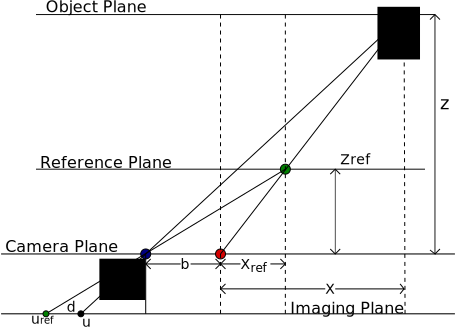
\includegraphics[width=0.8\textwidth]{DepthFromDisparity.png}
\caption{The geometry of converting disparity to depth.  The blue dot shows the location of the IR camera and the red dot shows the location of the IR projector.  The focal length is $f$ and the baseline (separation between IR camera and IR projector) is $b$.  Images are formed through the pinhole at the IR camera (blue dot) on the imaging plane, and the actual scene is above the camera plane.  The green dot is the location of a part of the dot pattern on the reference plane, while the black dot is the same part of that pattern on another plane further away.  $X_{\text{ref}}$ is the horizontal distance of the reference point from the IR projector, and $Z_{\text{ref}}$ is the depth of the reference point.  $Z$ is the depth of the actual point that is being measured, and $X$ is the horizontal distance of that point from the IR projector}
\label{fig:DepthFromDisparity}
\end{figure}



\bibliographystyle{plain}
\bibliography{KinectMath}

\end{document}
